% 图 78.1 —— 由 `checks/emit_hand.py` 自动拼出（probe 精测 + prims2 图元分解）
%%
% ⚠ 这是**稿子不是成品**：跑 `checks/checkhand.py 78.1` 看指标 + 看叠合图。
%%
%% ⚠ 待核：
%   · 本图 probe 报出阴影族 1 个 —— **本脚本不生成阴影**（要照原书手写）；prims2 的 strokes 里可能含阴影线，核对时留意别画重
%   · 可疑字形 1 项（空心圈 ⊙ 常被认成字母 o）—— 见文件末
%%
\documentclass[12pt]{standalone}
\usepackage{fontspec}
\setsansfont{Arial}
\newfontfamily\mfallback{DejaVu Sans}
\usepackage{tikz}
\begin{document}
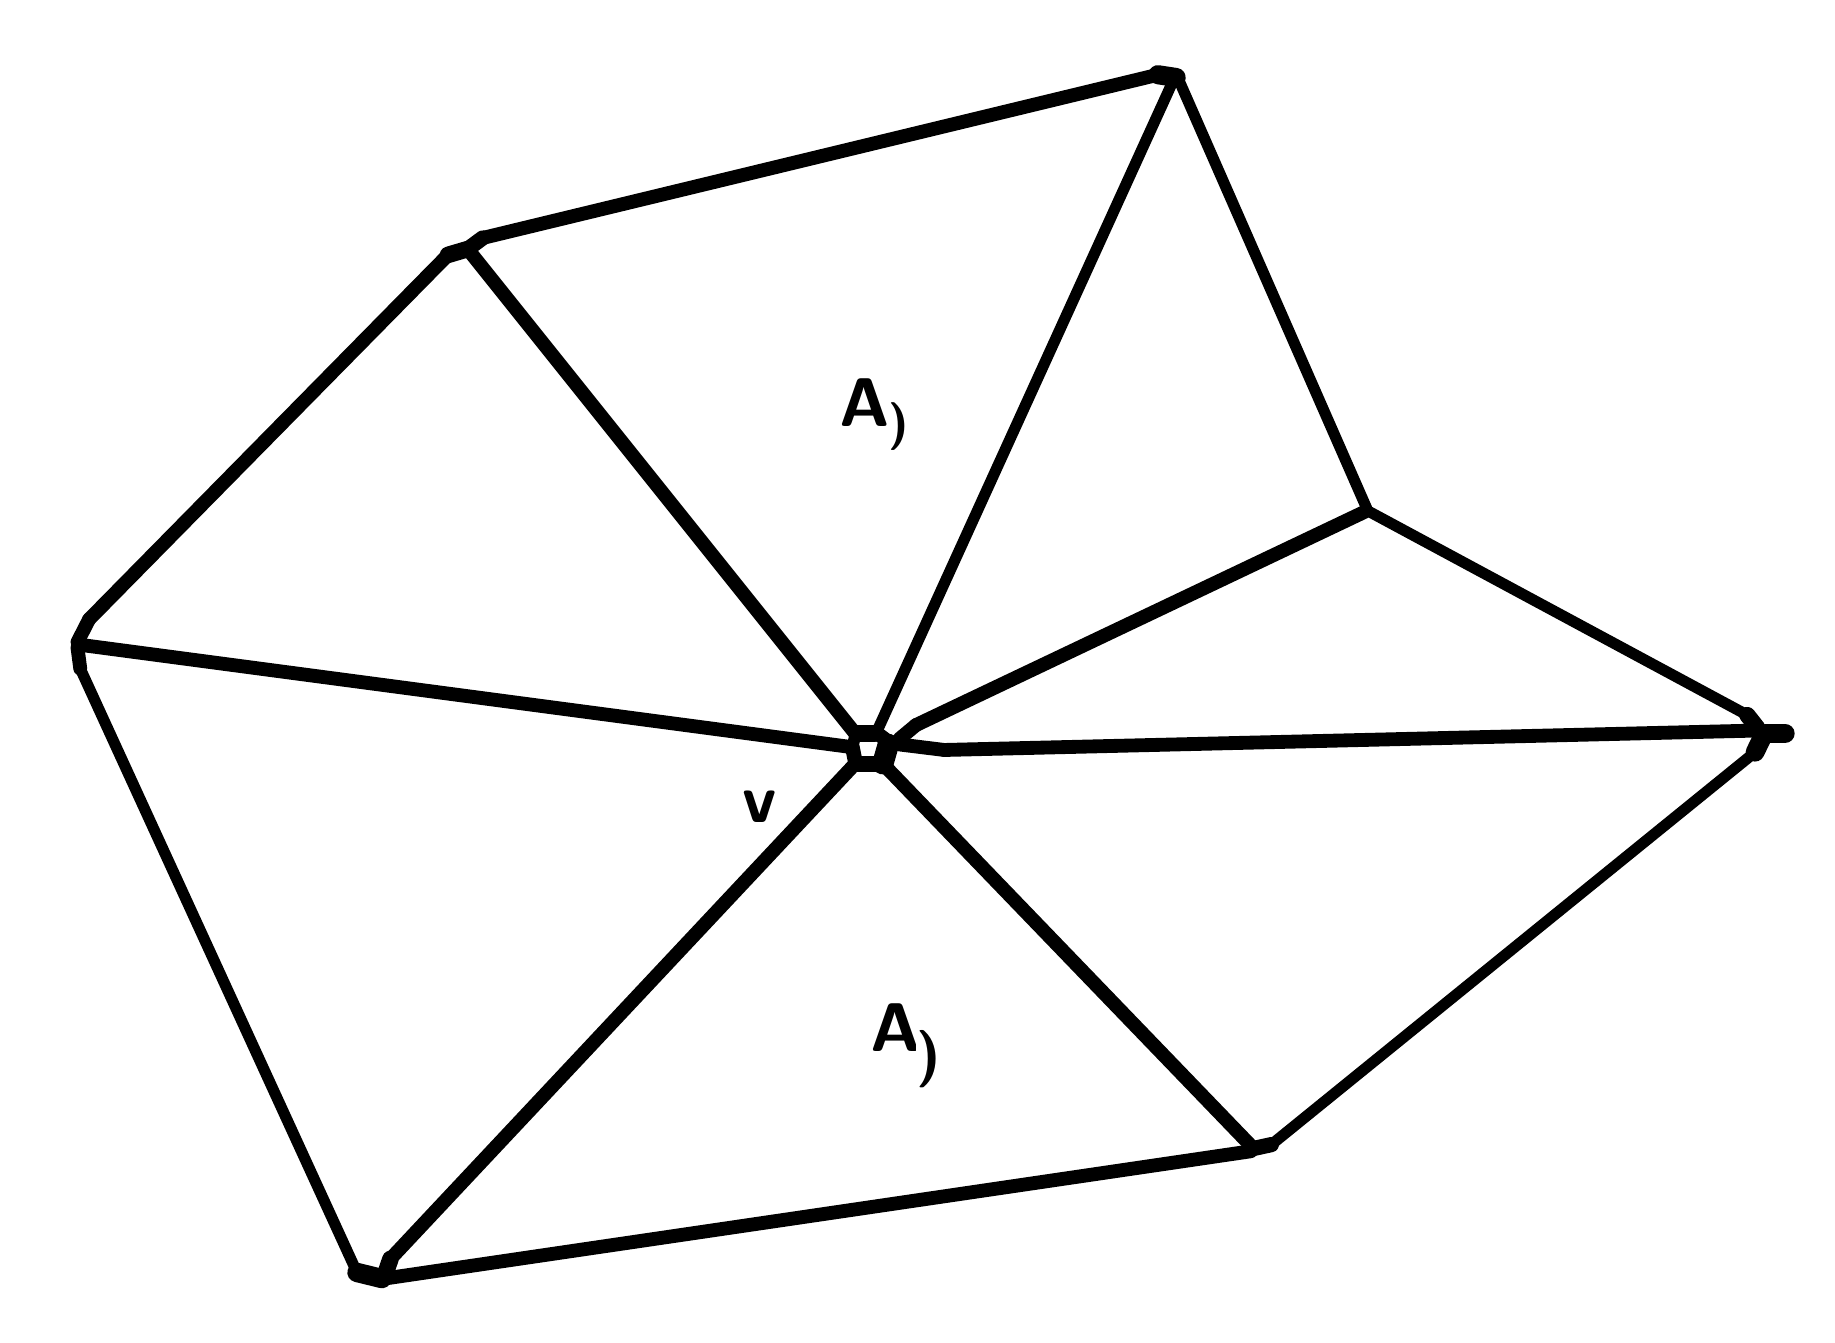
\begin{tikzpicture}[x=1pt, y=-1pt, line width=5.0pt, line cap=round, line join=round]

  %% ════ 直线段（prims2 的 strokes）════
  \draw[line width=5.0pt] (299.0,255.0) -- (159.0,80.0);
  \draw[line width=5.0pt] (483.0,175.0) -- (321.0,252.0);
  \draw[line width=5.0pt] (321.0,252.0) -- (315.0,257.0);
  \draw[line width=5.0pt] (129.0,452.0) -- (442.0,406.0);
  \draw[line width=5.0pt] (19.0,223.0) -- (298.0,260.0);
  \draw[line width=7.7pt] (311.0,259.0) -- (309.0,266.0);
  \draw[line width=5.0pt] (18.0,224.0) -- (19.0,231.6);
  \draw[line width=4.0pt] (19.0,231.6) -- (119.0,449.8);
  \draw[line width=7.0pt] (119.0,449.8) -- (128.0,452.0);
  \draw[line width=7.0pt] (628.0,255.0) -- (635.0,255.0);
  \draw[line width=5.5pt] (159.0,80.0) -- (164.4,76.0);
  \draw[line width=5.0pt] (164.4,76.0) -- (408.4,17.0);
  \draw[line width=6.9pt] (408.4,17.0) -- (415.0,18.0);
  \draw[line width=6.0pt] (159.0,80.0) -- (151.9,82.1);
  \draw[line width=5.0pt] (151.9,82.1) -- (22.2,213.8);
  \draw[line width=5.0pt] (22.2,213.8) -- (18.0,222.0);
  \draw[line width=4.0pt] (485.0,175.0) -- (621.4,248.4);
  \draw[line width=5.9pt] (621.4,248.4) -- (625.0,253.0);
  \draw[line width=5.3pt] (299.0,265.0) -- (298.0,260.0);
  \draw[line width=4.3pt] (299.0,256.0) -- (298.0,260.0);
  \draw[line width=5.0pt] (442.0,404.0) -- (309.0,266.0);
  \draw[line width=5.1pt] (307.0,255.0) -- (311.0,258.0);
  \draw[line width=4.0pt] (414.0,19.0) -- (307.0,254.0);
  \draw[line width=6.0pt] (300.0,266.0) -- (309.0,266.0);
  \draw[line width=6.0pt] (129.0,451.0) -- (131.1,444.9);
  \draw[line width=5.0pt] (131.1,444.9) -- (299.0,266.0);
  \draw[line width=5.5pt] (443.0,405.0) -- (449.4,403.6);
  \draw[line width=4.0pt] (449.4,403.6) -- (624.2,261.8);
  \draw[line width=6.8pt] (624.2,261.8) -- (627.0,256.0);
  \draw[line width=6.0pt] (300.0,255.0) -- (306.0,255.0);
  \draw[line width=4.0pt] (416.0,19.0) -- (484.0,174.0);
  \draw[line width=5.0pt] (624.0,254.0) -- (331.2,261.0);
  \draw[line width=5.0pt] (331.2,261.0) -- (315.0,259.0);

  %% ════ 标签（probe 直接给的 \node 行）════
  %% ⚠ 全部补了 fill=white：文字在最上层，否则与曲线交叉干扰
     \node[anchor=center,inner sep=0pt,fill=white,font=\fontsize{28.8}{36.0}\selectfont] at (302.6,135.5) {\textsf{\textbf{\textit{A}}}};   % box(291,124,18,22)
     \node[anchor=center,inner sep=0pt,fill=white,font=\fontsize{16.4}{20.5}\selectfont] at (314.8,144.3) {\textsf{\textbf{)}}};   % box(312,136,4,16)
     \node[anchor=center,inner sep=0pt,fill=white,font=\fontsize{29.5}{36.9}\selectfont] at (264.7,281.5) {\textsf{\textbf{\textit{v}}}};   % box(256,272,15,16)
     \node[anchor=center,inner sep=0pt,fill=white,font=\fontsize{28.8}{36.0}\selectfont] at (313.6,361.5) {\textsf{\textbf{\textit{A}}}};   % box(302,350,18,22)
     \node[anchor=center,inner sep=0pt,fill=white,font=\fontsize{21.0}{26.3}\selectfont] at (325.6,372.9) {\textsf{\textbf{)}}};   % box(322,362,5,21)

  % 钉死画布：否则超出的图元/控制点会把页面撑大，1:1 回比就失准
  \pgfresetboundingbox
  \path[use as bounding box] (0,0) rectangle (643,465);
\end{tikzpicture}
\end{document}

% ⚠ 待核清单（probe 拿不准，人眼过一遍）：
%   · 未识别/跳过：⑤ 跳过/未识别的字形
